\documentclass[a4paper,12pt]{article}
\usepackage{times}
\usepackage[francais]{babel}
\usepackage[utf8x]{inputenc}
\usepackage[T1]{fontenc}
\usepackage{amsmath}
\usepackage{amssymb}
\usepackage{graphicx}
\usepackage{pdfpages}
\usepackage{pdflscape}
\usepackage{listings}
\usepackage{longtable}
\lstset{literate=
{é}{{\'e}}1
{è}{{\`e}}1
{ê}{{\^e}}1
{à}{{\`a}}1
{â}{{\^a}}1
}
\lstset{language=C++,
                basicstyle=\footnotesize,
                keywordstyle=\footnotesize\color{blue},
                otherkeywords={override,nullptr}
}
\definecolor{orange}{rgb}{0.8,0.4,0.0}
\definecolor{darkblue}{rgb}{0.0,0.0,0.6}
\definecolor{cyan}{rgb}{0.0,0.6,0.6}
\lstdefinelanguage{JSON}
{
  basicstyle=\normalsize,
  columns=fullflexible,
  showstringspaces=false,
  commentstyle=\color{gray}\upshape,
  morestring=[b]",
  morestring=[s]{>}{<},
  morecomment=[s]{<?}{?>},
  stringstyle=\color{orange},
  identifierstyle=\color{darkblue},
  keywordstyle=\color{blue},
  morekeywords={string,number,array,object}% list your attributes here
}

\sloppy

\setlength{\topmargin}{0cm}
\setlength{\headsep}{0.in}
\setlength{\headheight}{0.in}
\setlength{\evensidemargin}{0cm}
\setlength{\oddsidemargin}{-1cm}
\textwidth 18cm
\textheight 25cm

\begin{document}

\thispagestyle{empty}

\begin{titlepage}

\vspace*{2cm}

\begin{center}\textbf{\Huge Projet Logiciel Transversal}\end{center}{\Large \par}

\begin{center}\textbf{\large JAMET Romain DORRA Benjamin}\end{center}{\large \par}

\vspace{2cm}

%\begin{figure}[h]
%\begin{center}
%\includegraphics[width=\textwidth]{exemple.png}
%\caption{\label{pacmangame}Exemple du jeu}
%\end{center}
%\end{figure}

\clearpage

{\small
\tableofcontents
}

\end{titlepage}

\clearpage
\section{Présentation Générale}

\subsection{Archétype}
Le jeu d’origine est le jeu de stratégie/gestion Crusader Kings II, développé et édité par le studio Paradox Interactive. 

Il s’agit d’un jeu se déroulant dans l’Europe et le Moyen-Orient entre le VIIIe et le XVe siècle, où les joueurs jouent le rôle d’une dynastie de nobles régnant sur un domaine, qu’ils peuvent faire croitre par une mécanique de titres de noblesse, de guerre et de diplomatie inspirés du Moyen-Âge. 
Les règles en seront bien évidemment simplifiées dans le cadre du projet. 

Le descriptif des règles ci-dessous présente le projet tel qu’il devrait être au final. \\

\subsection{Règles du jeu}
Les joueurs sont des nobles qui règnent sur ces provinces, en possédant un ou plusieurs titres de noblesse. Les trois titres sont, dans l'ordre du plus puissant au moins puissant : les Rois, les Ducs, et les Comtes.

À chaque province est lié un titre de Comte. Posséder un titre de Comte, c'est posséder la province associée. 

Une province possède plusieurs caractéristiques décrivant son niveau de développement, son état de dévastation ou de prospérité, qui influent sur les impôts qu'elle génère, et les levées militaires qu'elle peut supporter. Un Comte peut posséder plusieurs Comtés, cependant, le nombre en est limité. Si cette limite est dépassée, un malus d’impôts et de levées est appliqué.  \\

Un Duc est plus puissant qu’un Comte. Pour pouvoir contrôler plus de territoire malgré la limite mentionnée précédemment, il doit confier la gestion de certaines provinces à des nobles qui seront ses vassaux. 

Un Duc ne peut avoir que des Comtes pour vassaux.

Un Roi est plus puissant qu’un Duc. Il peut avoir comme vassaux des Ducs et des Comtes.
Lorsqu’un seigneur est vassal, il paie un impôt en or et en hommes à son suzerain. \\

Pour faire la guerre à son voisin, il faut un Casus Belli. Il y aura la possibilité de dépenser de l’or pour fabriquer une revendication à un titre de Comte, pour essayer de s’en emparer à la guerre. Une fois la guerre déclarée, on peut mobiliser les troupes dans les provinces que l’on possède, ainsi que les troupes de ses vassaux si on en a, et leur donner des ordres de déplacement sur la carte.

Lorsque deux armées hostiles se rencontrent, un combat a lieu. L’armée défaite est mise en déroute et cherchera automatiquement à revenir à sa province d’origine. \\

Chaque Comté fait partie d’un Duché «de Jure », c’est-à-dire un Duché dont le titre n’existe pas, mais qui peut être créé si quelqu’un en contrôle plus de la moitié et dépense une certaine somme. Le fait de posséder un titre de Duc offre un Casus Belli permettant de vassaliser les Comtes dont les terres font partie « de Jure » de votre Duché.

De même, chaque Duché fait partie d’un Royaume de Jure. Posséder ou contrôler par le biais de vassaux une certaine proportion d’un Royaume de Jure vous permet de créer ce titre en échange d’argent. Posséder un tel titre offre un Casus Belli contre tous les Ducs et Comtes faisant partie de Jure de votre Royaume.
On peut bien évidemment posséder ou contrôler par vassaux des provinces n’appartenant pas de Jure à votre domaine. \\

Il est possible d’interagir avec d’autres personnages, forger des alliances, des pactes de non-agression, proposer à un seigneur plus faible de devenir votre vassal. 

Chaque personnage possède un score décrivant son opinion envers les autres, influencé par l’historique de leurs actions. Ce score permettra de définir le comportement de l’IA. Il sera également influencé par des traits de personnalité des personnages.
L’IA prendra ses décisions en utilisant une mécanique de MMTH (mean time to happen, ou temps moyen d’attente). Pour chaque action, il y a un MTTH en nombre de tours, avec des modificateurs liés aux traits de personnalité aléatoires des personnages.

Au cours de son règne, un personnage accumule des points de prestige selon la quantité de titres qu’il possède, ainsi que les titres de ses vassaux. Lorsqu’il meurt, un héritier apparaît, et le score de prestige s’ajoute au score du joueur. Le score final d’un joueur correspond donc à la somme de points de prestige accumulés par tous les seigneurs successifs qu’il a joué. \\


\subsection{Ressources}
Pour réaliser ce projet, nous aurons besoin en termes de ressources d’une carte du monde du jeu, avec les différentes provinces découpées. 

Nous aurons besoin d’une version pour l’affichage, et d’une autre qui ne sera pas affichée pour identifier la province sur laquelle le joueur clique, par un code couleur unique par province. \\

Nous aurons besoin de sprites d’armée immobile, en mouvement, et à la bataille. 

Nous devrons pouvoir coloriser facilement les bannières pour identifier immédiatement le contrôleur de l’armée. 

Nous pouvons également avoir besoin d’images pour les personnages, même si ce n’est pas obligatoire il s’agirait d’un plus. Dans le même ordre d’idées, nous pourrions employer diverses images sur le thème médiéval pour illustrer les différents menus du jeu. Nous pouvons aussi utiliser différentes musiques d’ambiance, des bruitages de bataille, et quelques sons génériques pour l’appui sur les boutons de l’interface. \\

\clearpage
\section{Description et conception des états}

\subsection{Description des états}


\subsection{Conception Logiciel}


%\begin{landscape}
%\begin{figure}[p]
%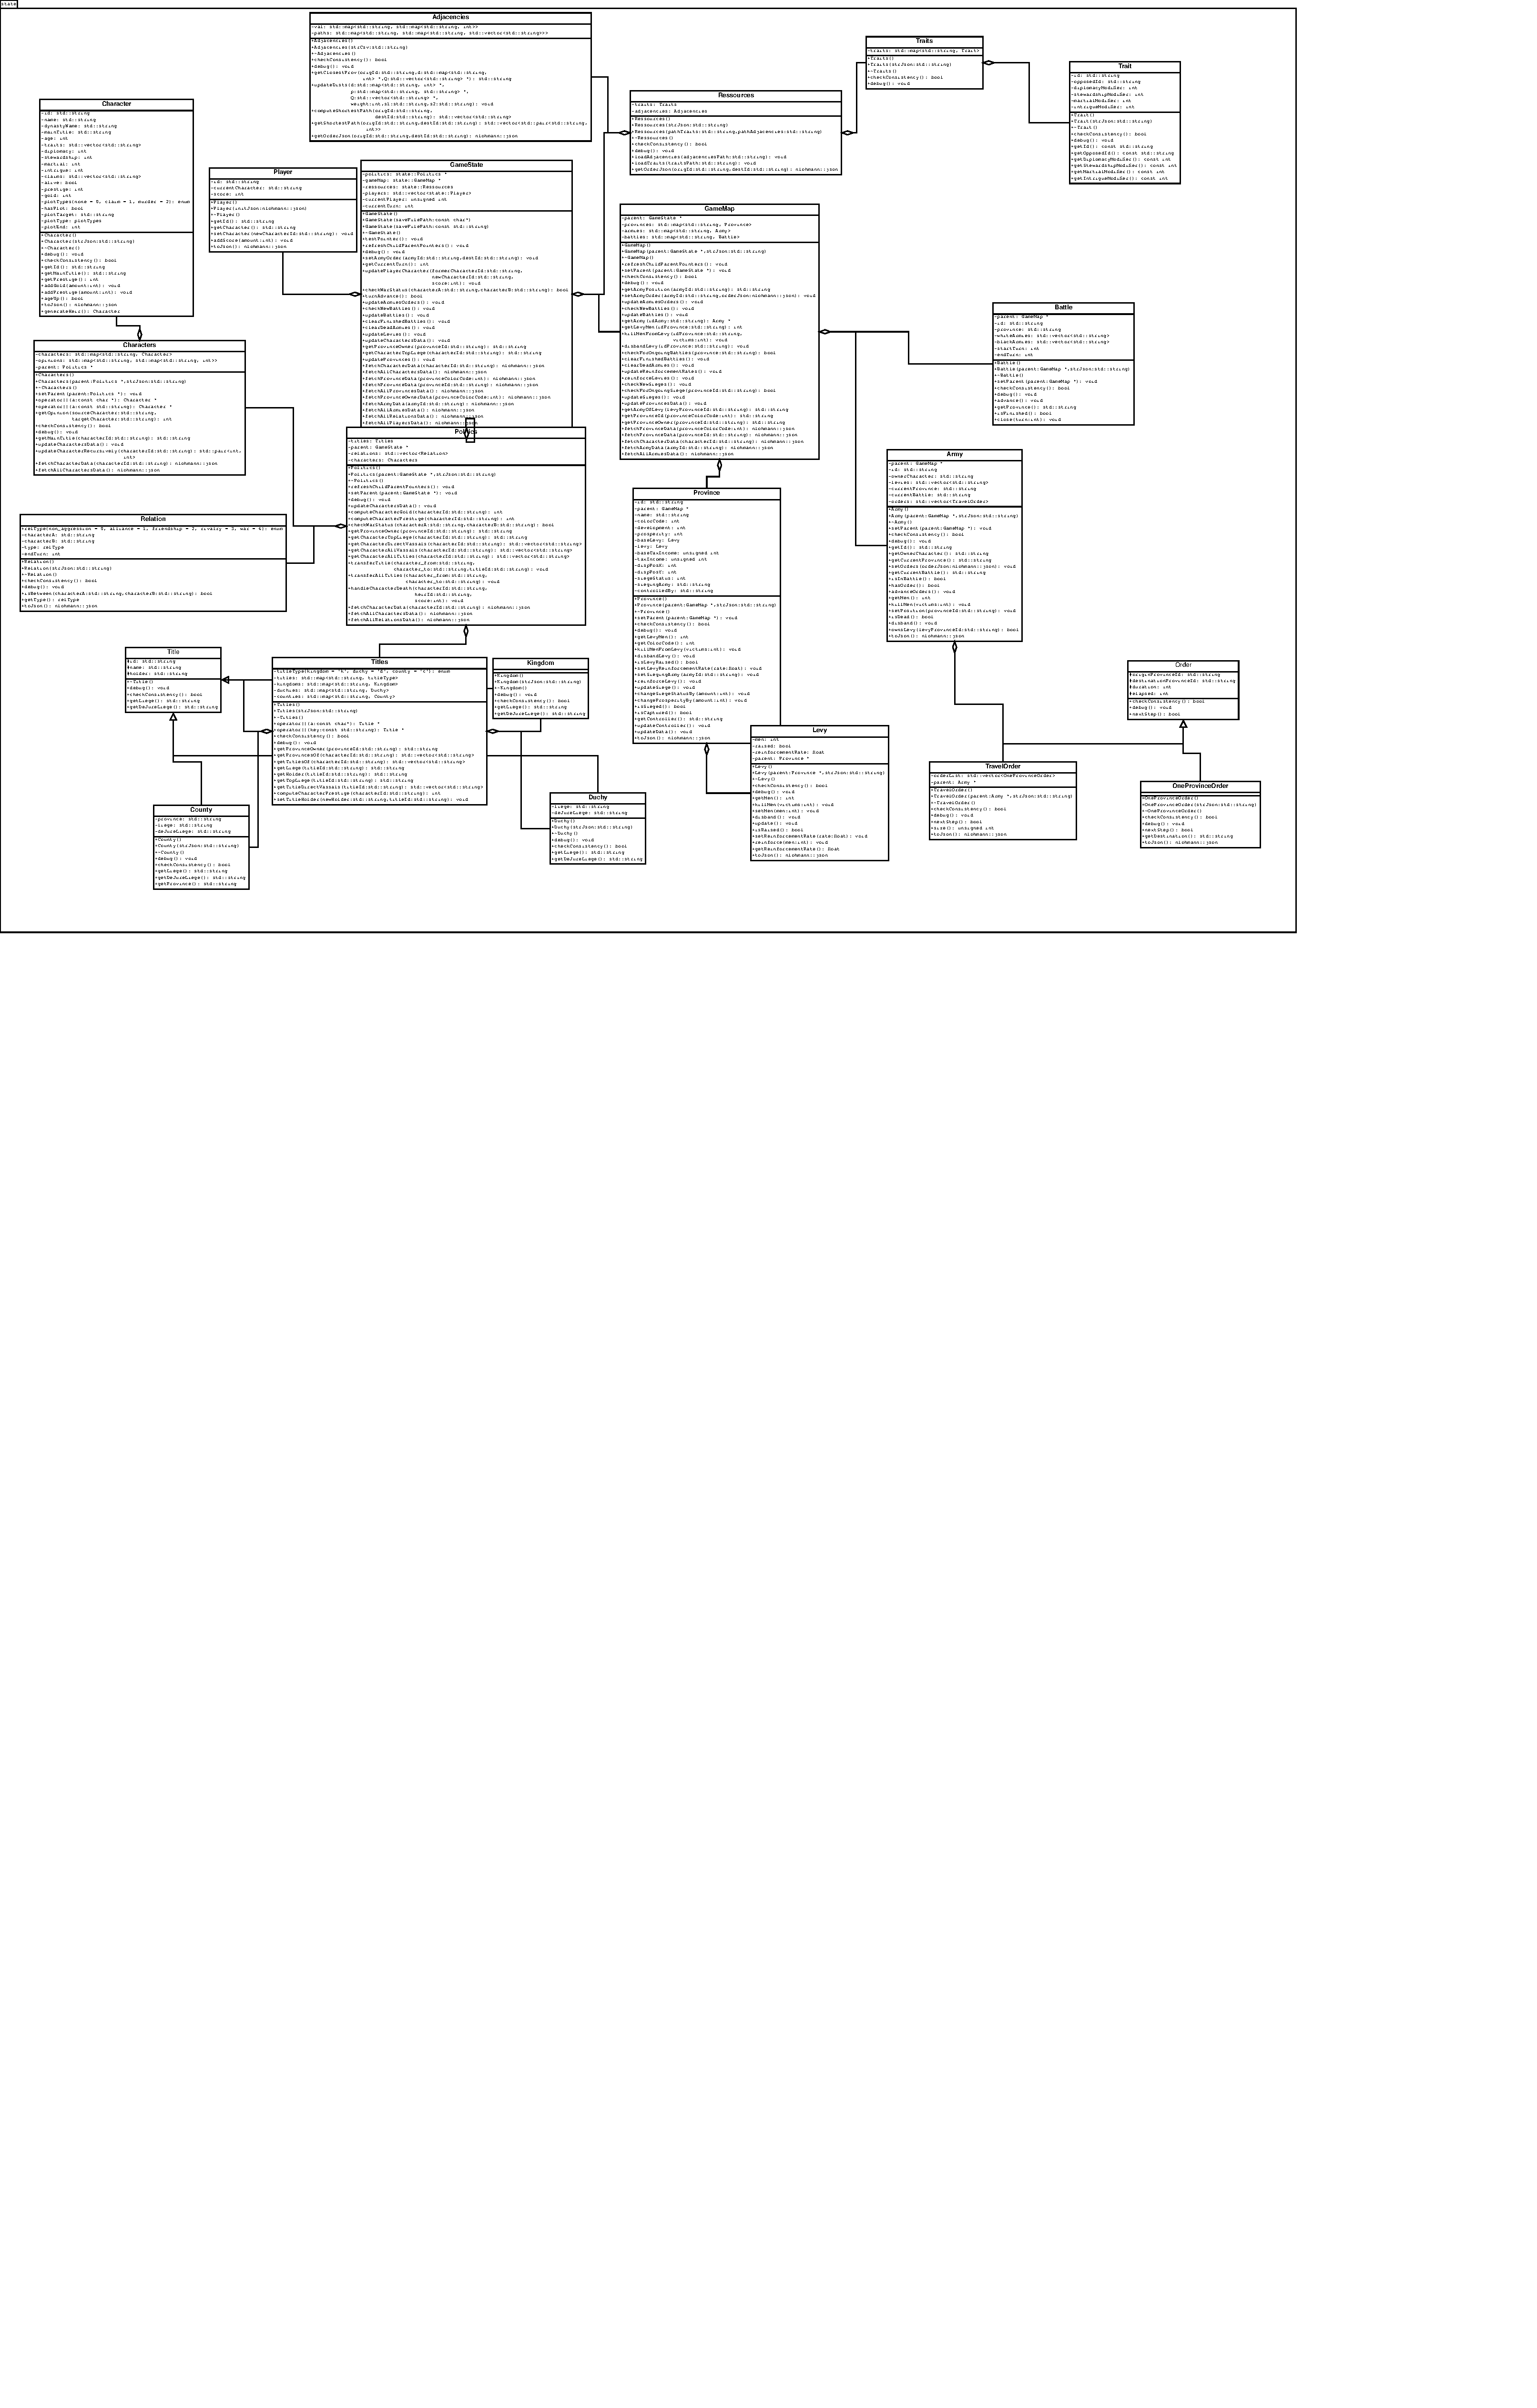
\includegraphics[width=0.9\paperheight]{state.pdf}
%\caption{\label{uml:state}Diagramme des classes d'état.} 
%\end{figure}
%\end{landscape}

\clearpage
\section{Rendu: Stratégie et Conception}

\subsection{Stratégie de rendu d'un état}


\subsection{Conception logiciel}

%\begin{landscape}
%\begin{figure}[p]
%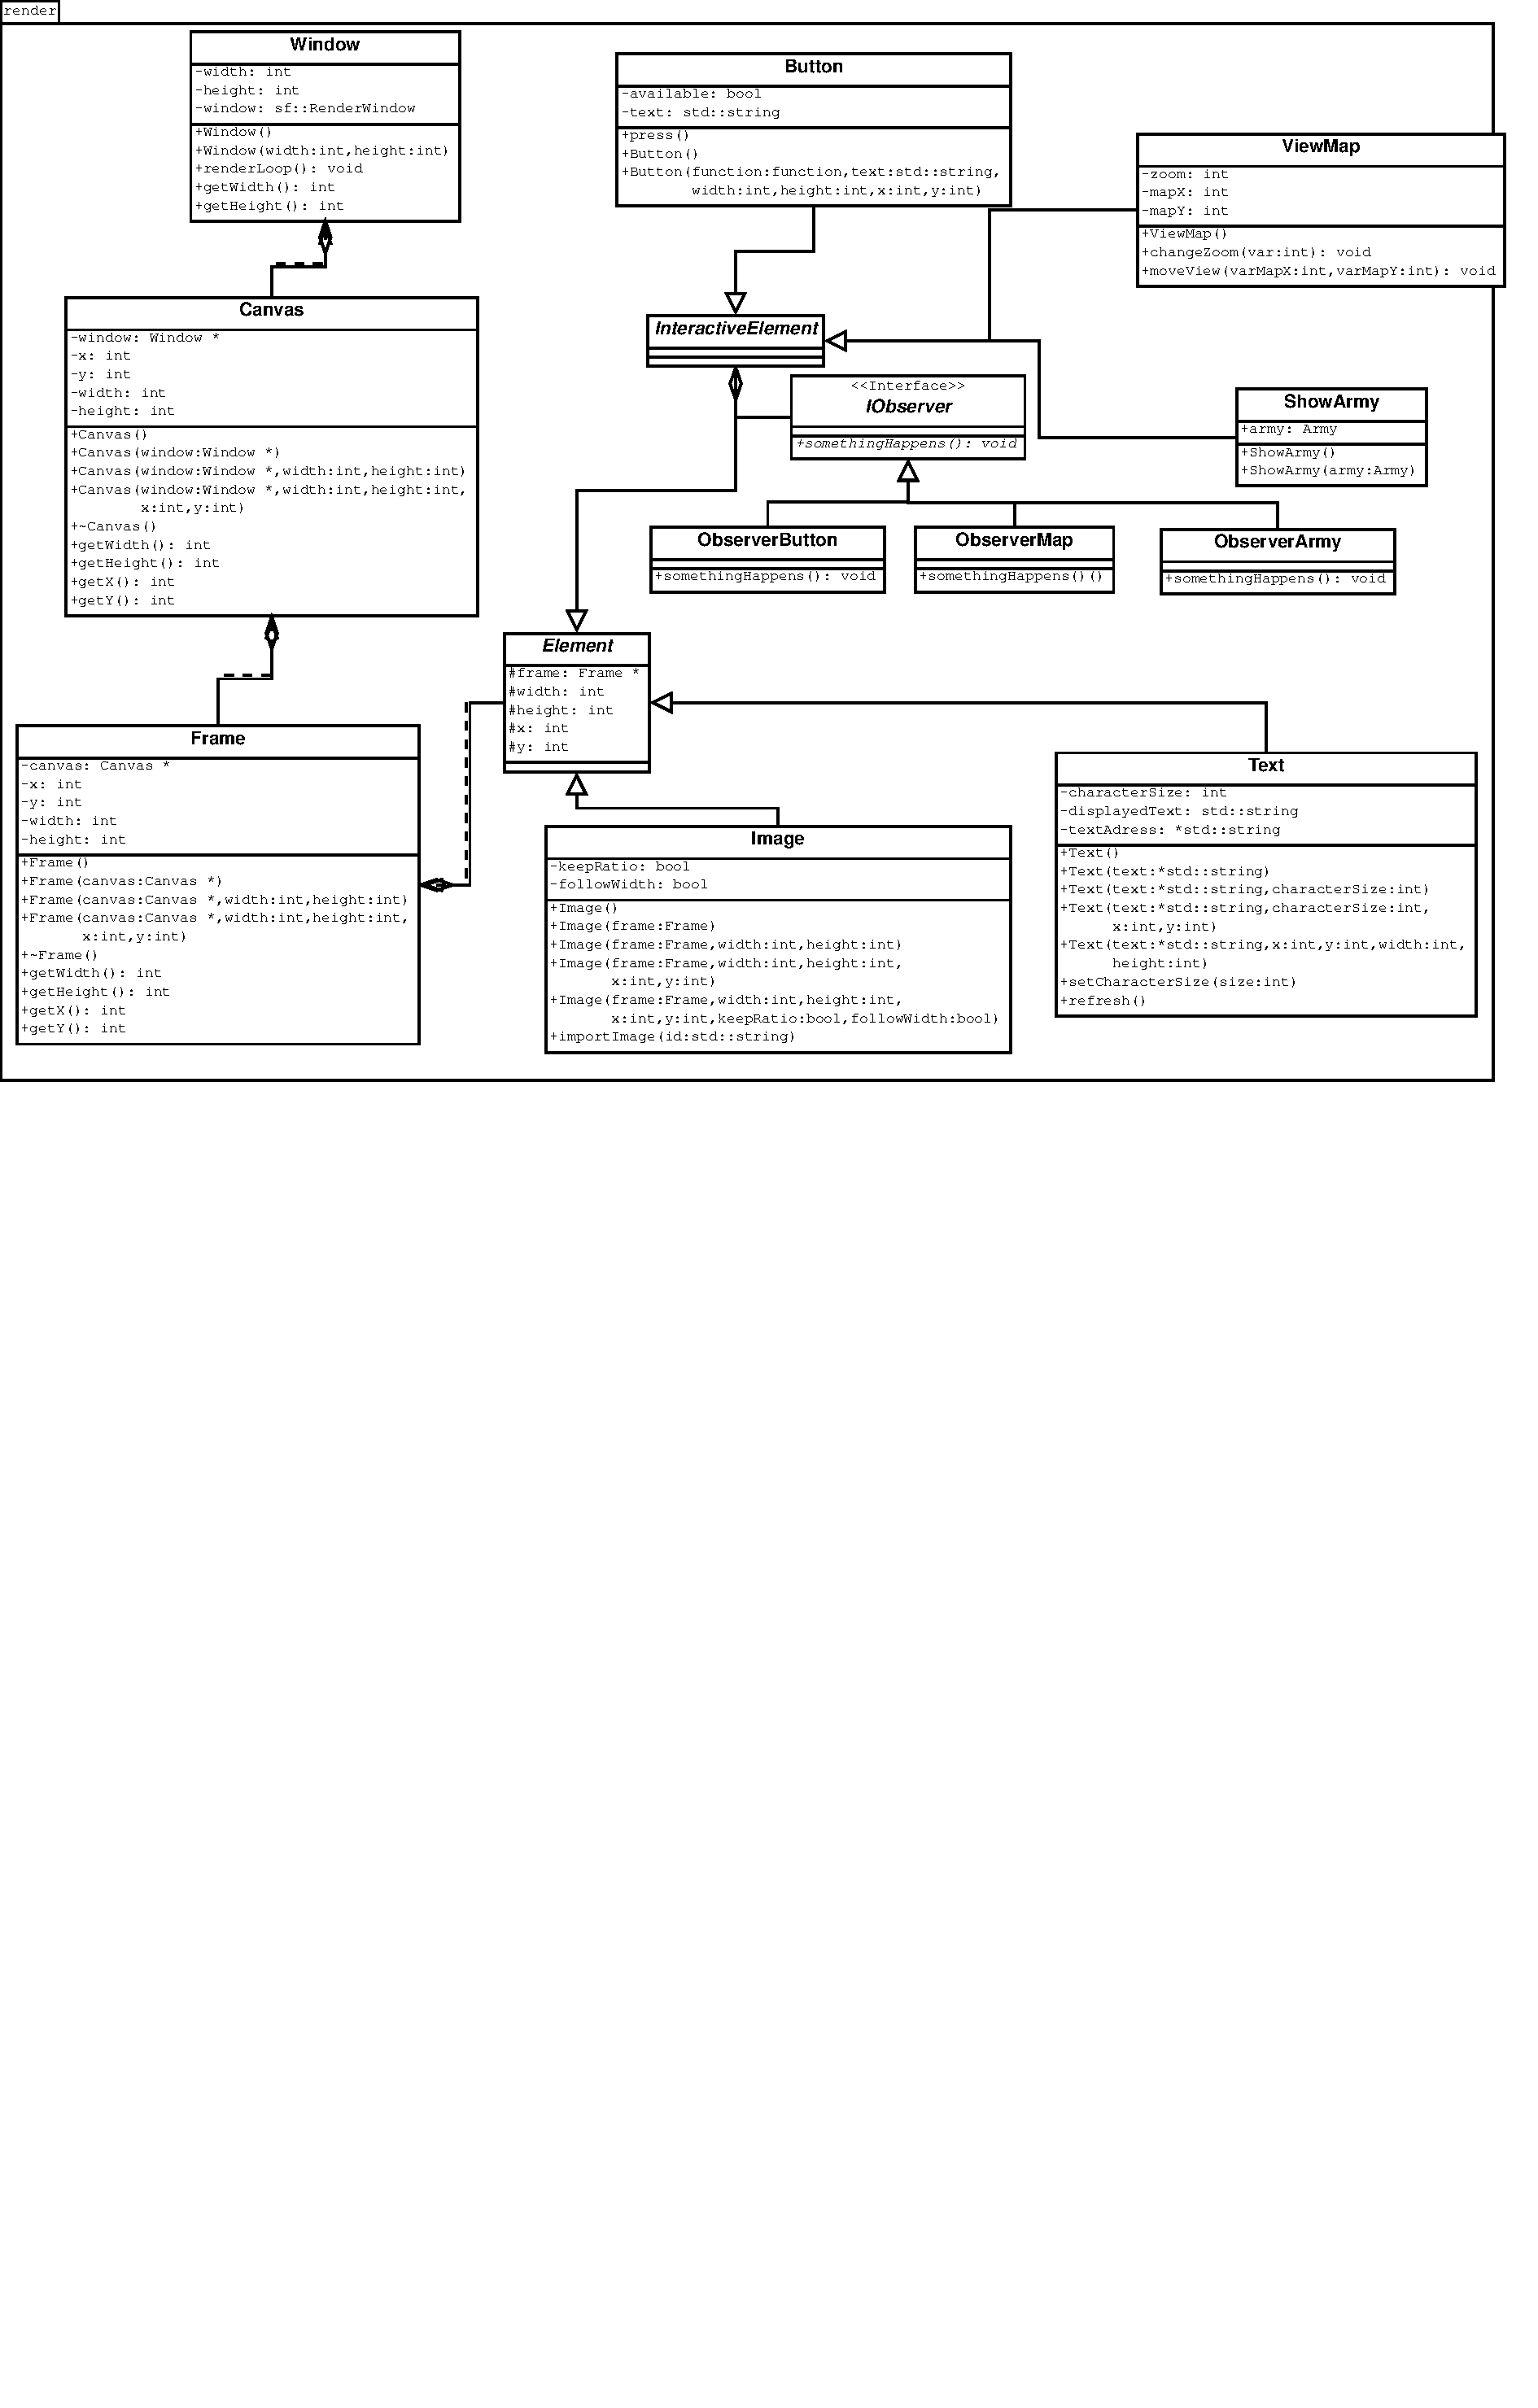
\includegraphics[width=0.9\paperheight]{render.pdf}
%\caption{\label{uml:render}Diagramme des classes de rendu.} 
%\end{figure}
%\end{landscape}

\clearpage
\section{Règles de changement d'états et moteur de jeu}

\subsection{Règles}

\clearpage
\subsection{Conception logiciel}


%\begin{landscape}
%\begin{figure}[p]
%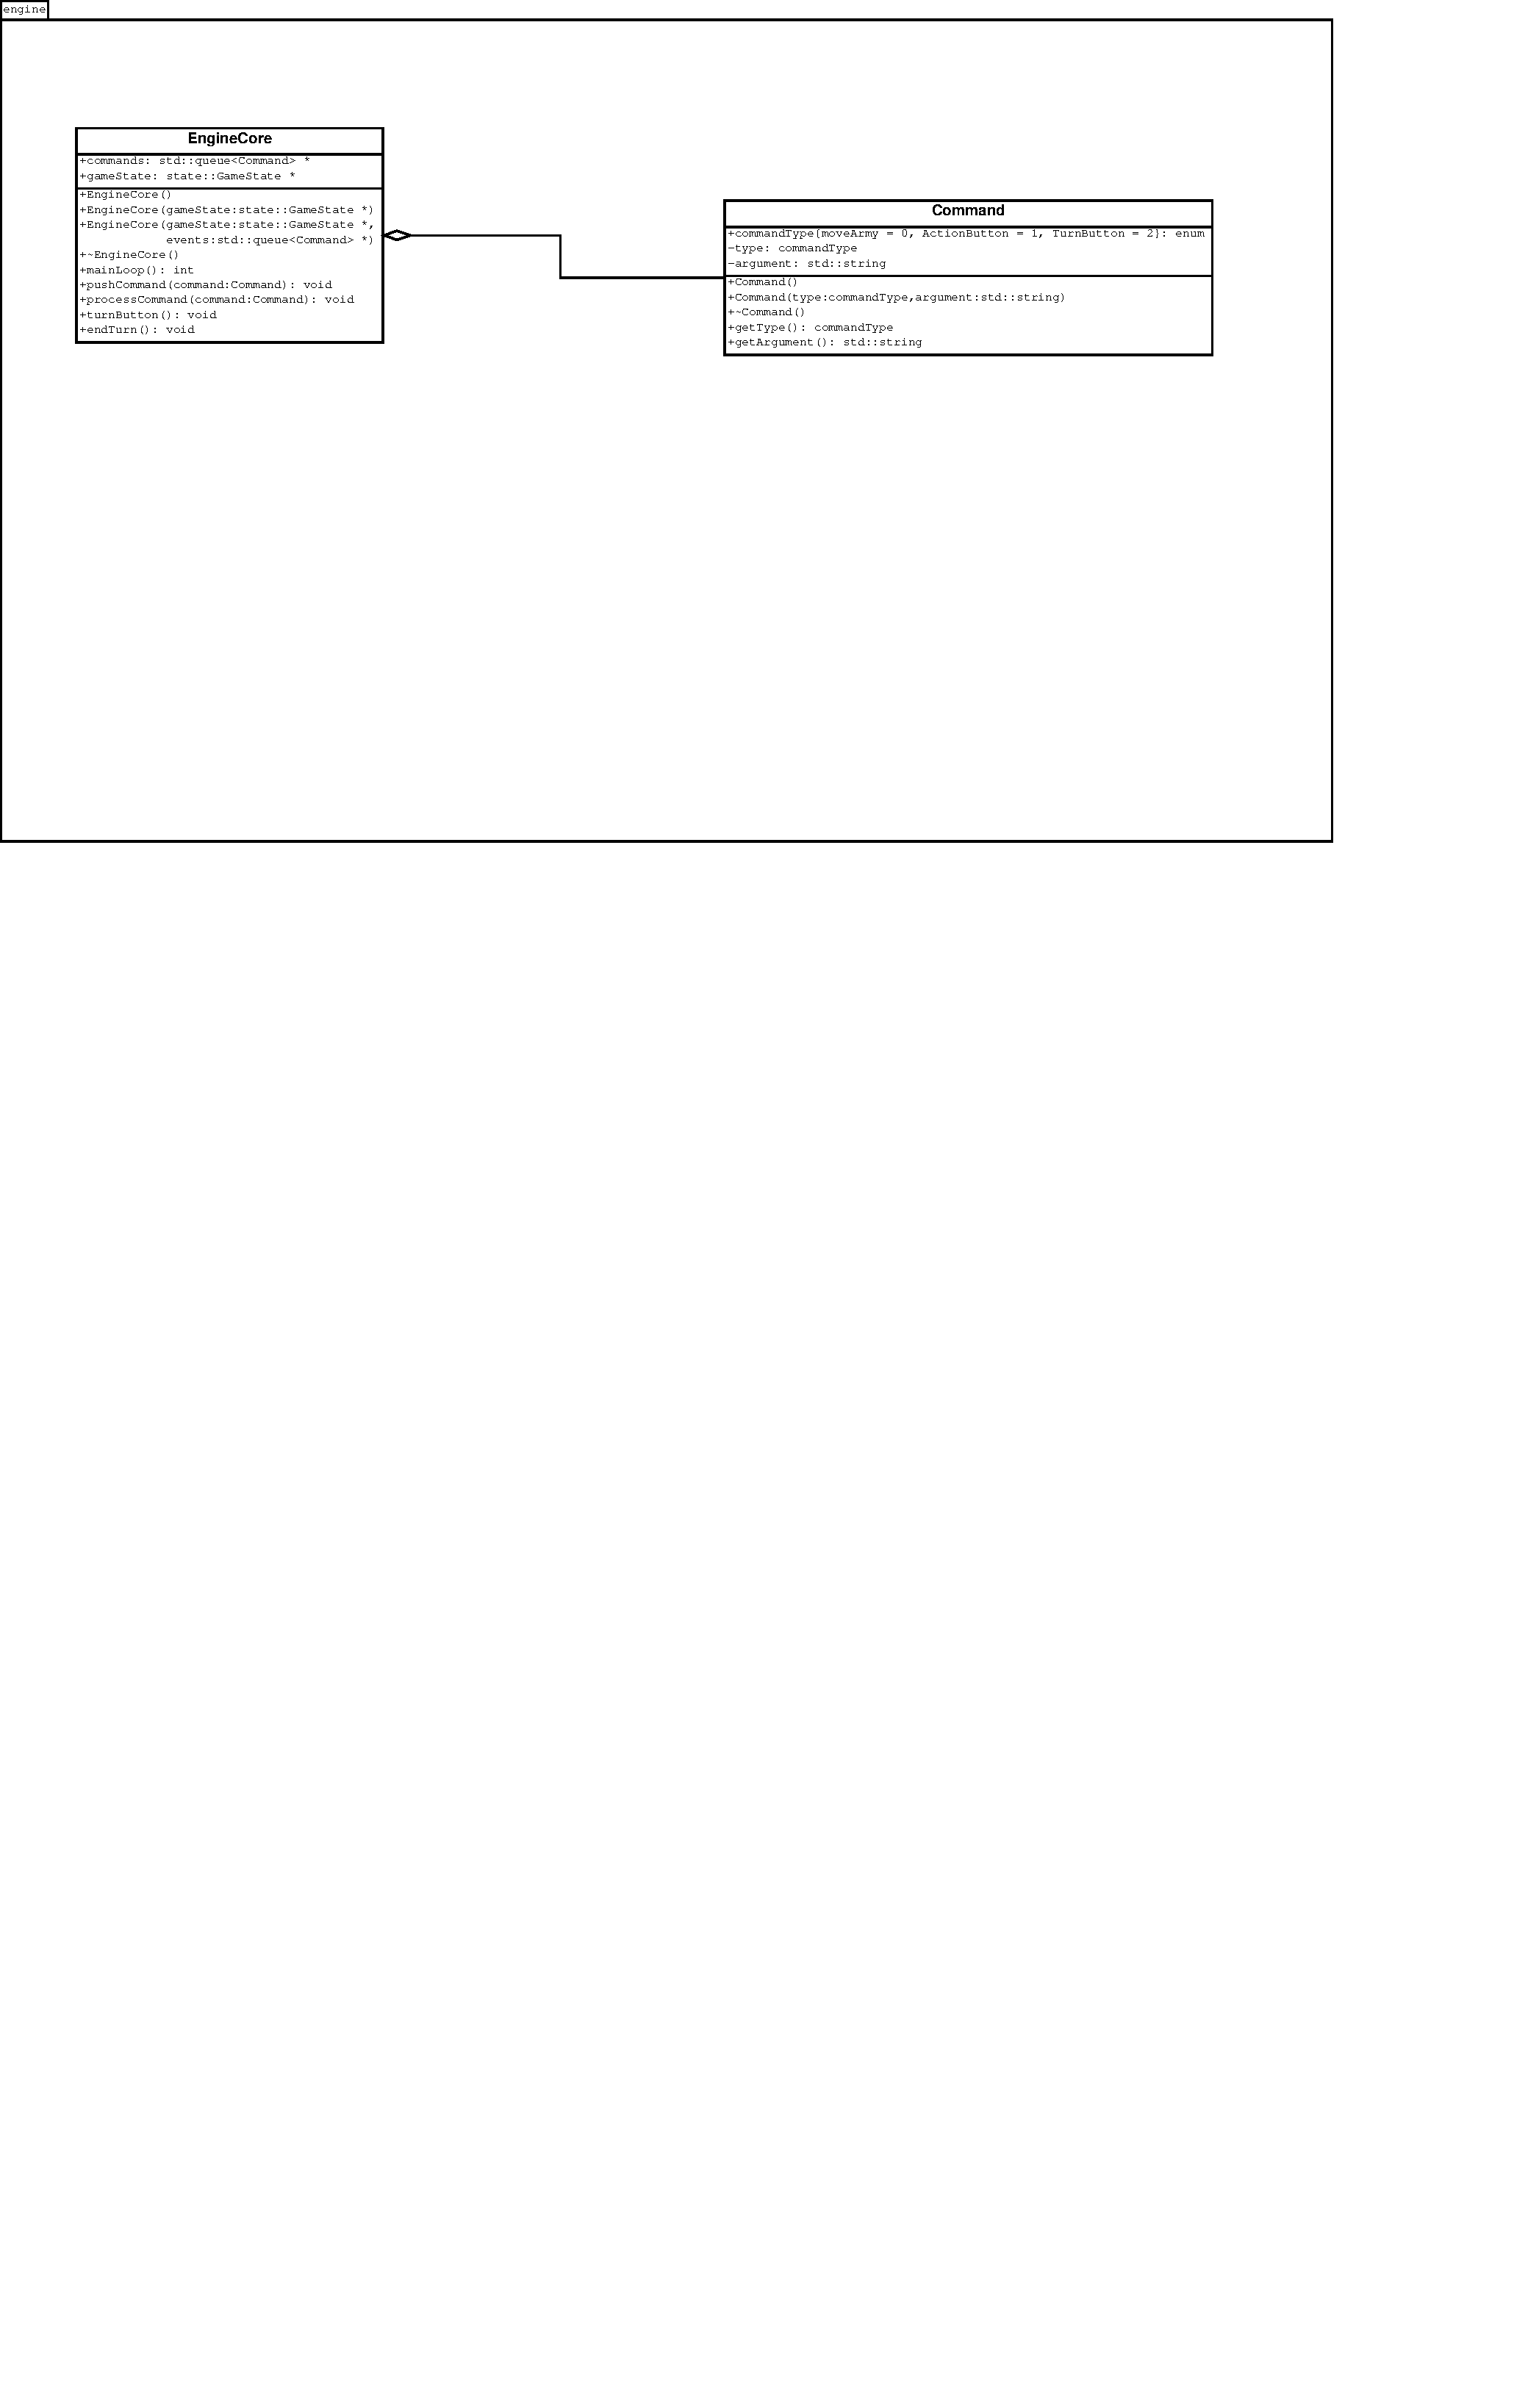
\includegraphics[width=0.9\paperheight]{engine.pdf}
%\caption{\label{uml:engine}Diagramme des classes de moteur de jeu.} 
%\end{figure}
%\end{landscape}


\section{Intelligence Artificielle}

\subsection{Stratégies}

\clearpage
\subsection{Conception logiciel}


%\begin{landscape}
%\begin{figure}[p]
%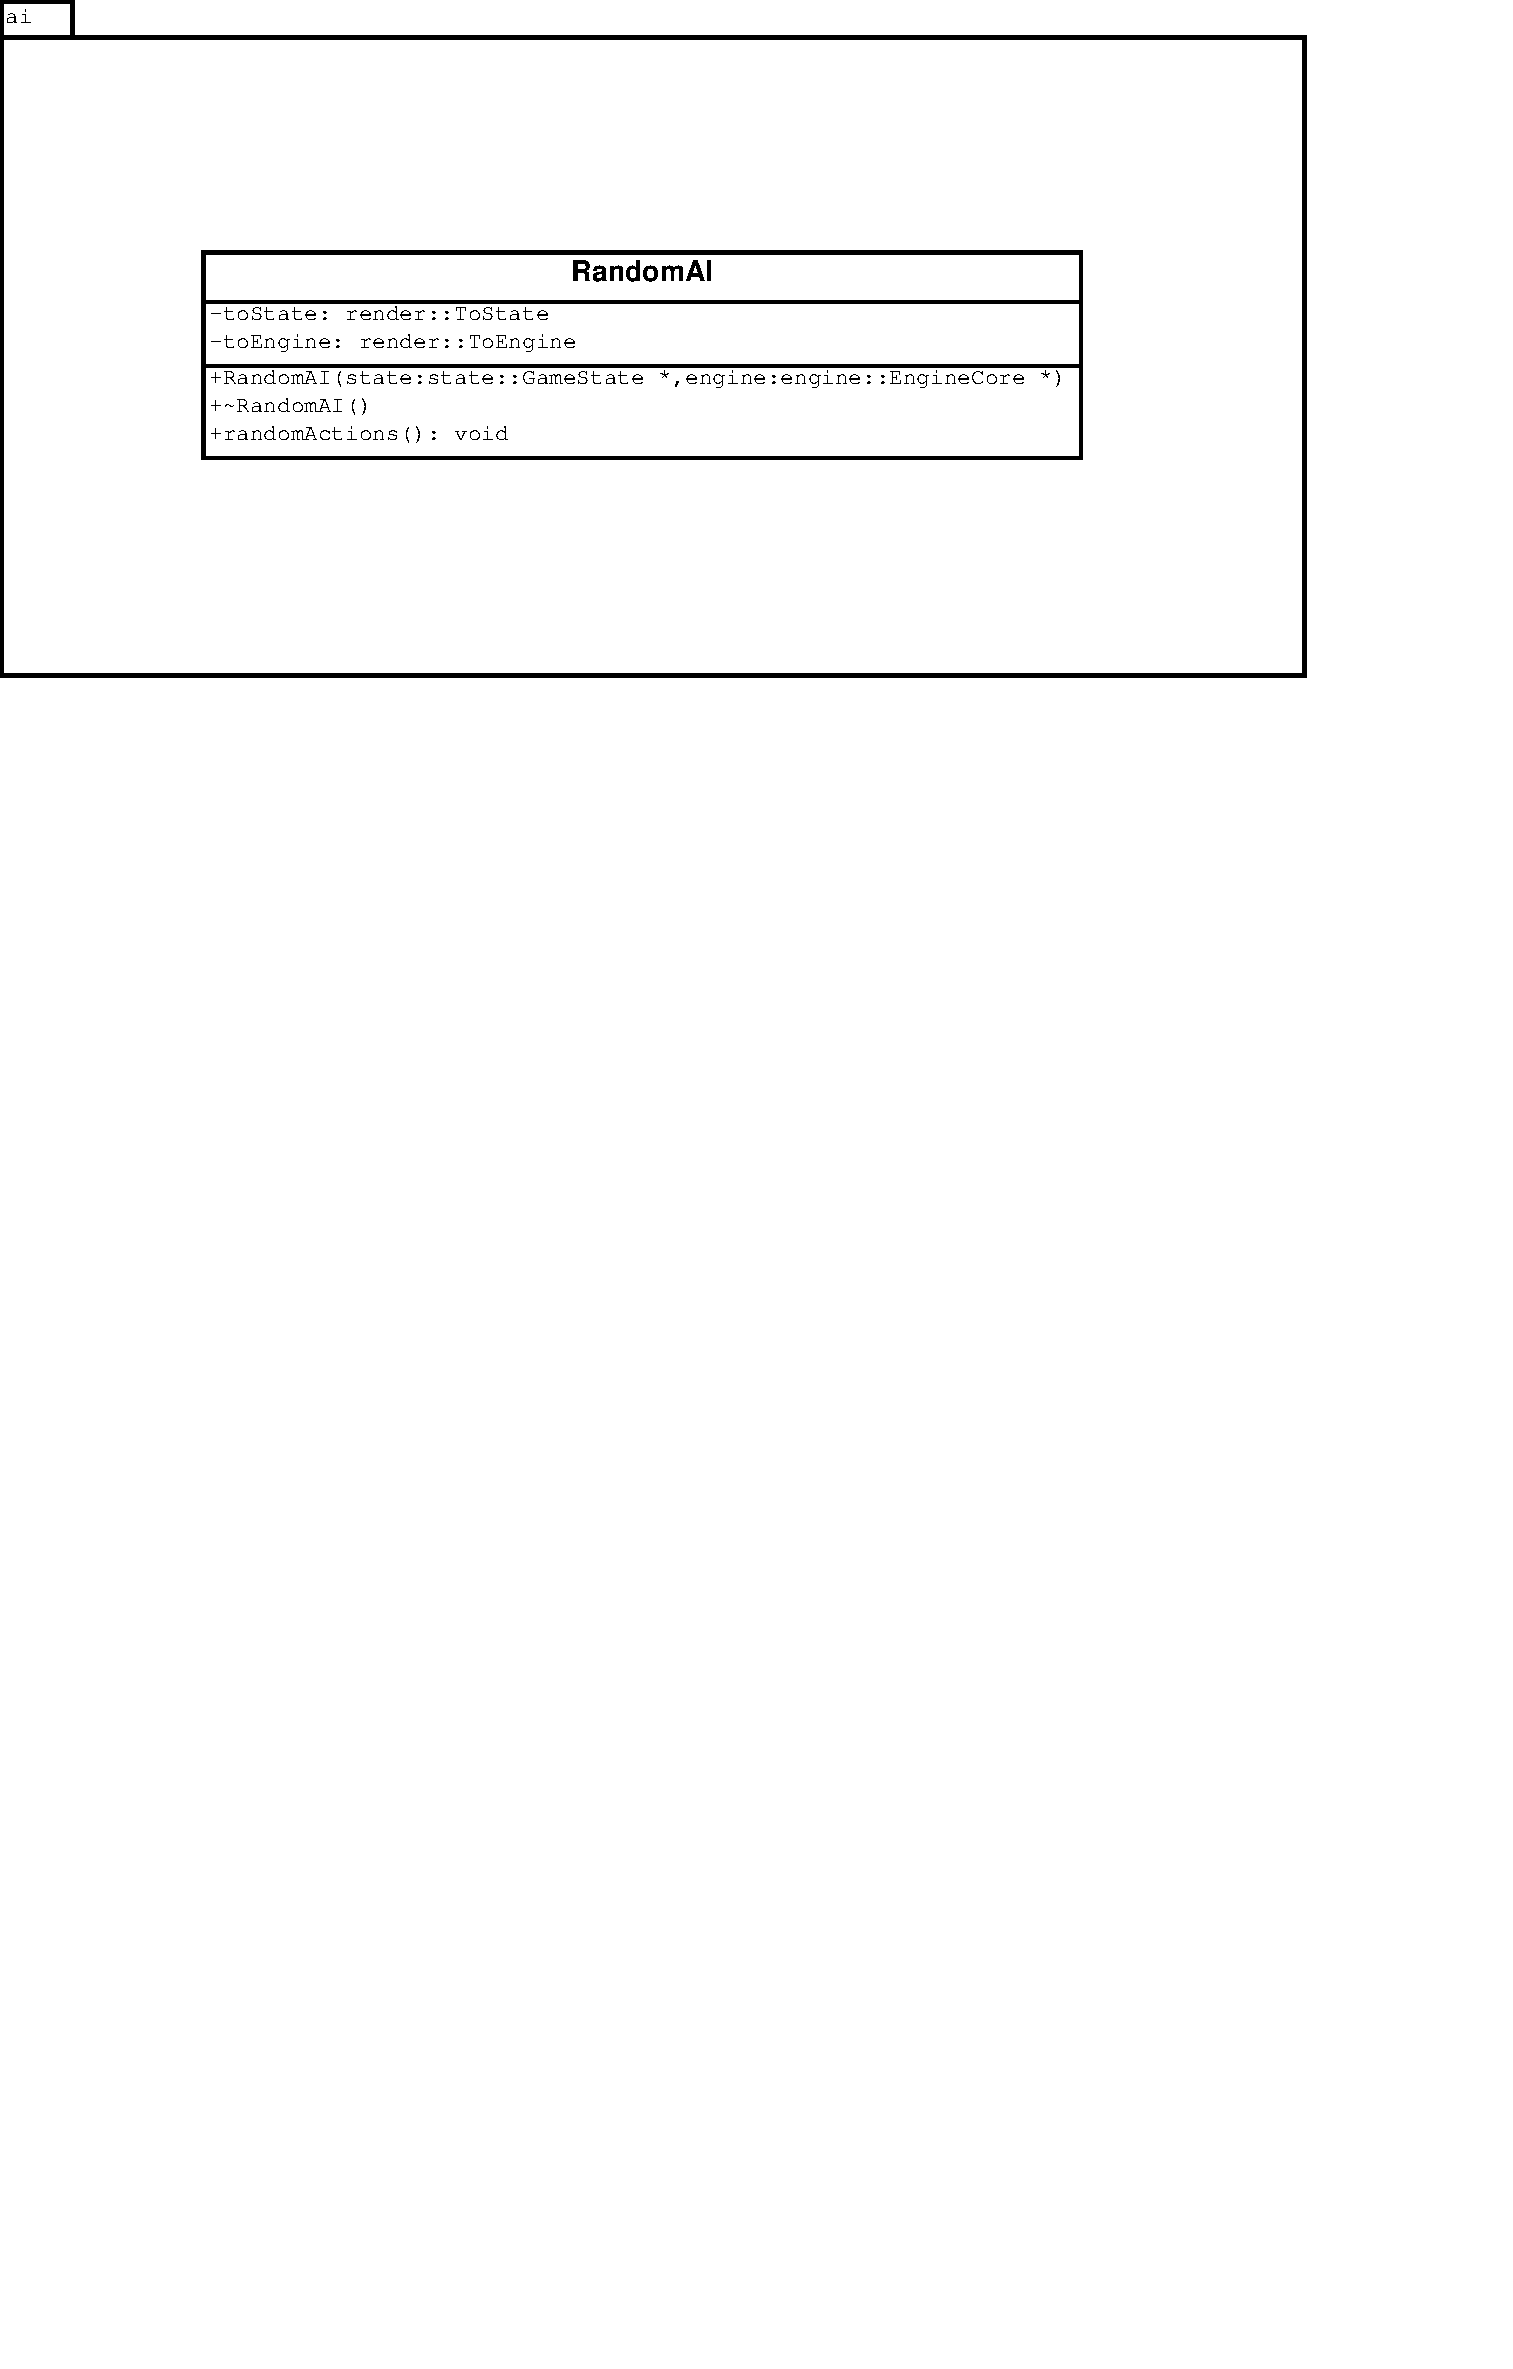
\includegraphics[width=0.9\paperheight]{ai.pdf}
%\caption{\label{uml:ai}Diagramme des classes d'intelligence artificielle.} 
%\end{figure}
%\end{landscape}


\section{Modularisation}
\label{sec:module}

\subsection{Organisation des modules}

\clearpage
\subsection{Conception logiciel}


%
%\begin{landscape}
%\begin{figure}[p]
%\includegraphics[width=0.9\paperheight]{module.pdf}
%\caption{\label{uml:module}Diagramme des classes pour la modularisation.} 
%\end{figure}
%\end{landscape}

\end{document}
